\documentclass[tikz, convert=pdf2svg]{standalone}

\usetikzlibrary{positioning, backgrounds, calc}
\begin{document}
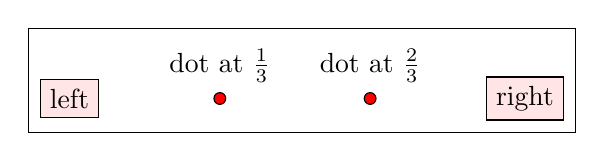
\begin{tikzpicture}[framed]
    \node[draw, fill=red!10] (left) {left};
    \node[draw, fill=red!10, right=140pt of left] (right) {right};
 
    \node[draw, inner sep=1.5pt, circle, fill=red, label={dot at $\frac{1}{3}$}] at ($(left)!0.33!(right)$) {};
    \node[draw, inner sep=1.5pt, circle, fill=red, label={dot at $\frac{2}{3}$}] at ($(left)!0.66!(right)$) {};
\end{tikzpicture}
\end{document}
